\setcounter{chapter}{0}
\chapter{Automaton}
\begin{definition} ~
    \begin{itemize}
        \item Define the \textbf{alphabet} $\Sigma$ as the set of symbols, usually take $\Sigma = \{ 0,1 \}$.
        \item Define a \textbf{string} as a finite sequence of symbols from $\Sigma$.
        \item Define $\Sigma^{*} = \bigcup_{i \ge 0} \Sigma^{i}$, where $\Sigma^{i}$ denotes the set of strings with length $i$. $\Sigma^{*}$ is the set of all string over the \textbf{alphabet} $\Sigma$.
        \item Define a \textbf{language} $L$ as a subset of $\Sigma^{*}$.
    \end{itemize}
\end{definition}
\begin{eg} ~
\begin{itemize} 
    \item $\{ 0,1 \}^{2} = \{ 00, 01, 10, 11 \}$.
    \item $\{ 0,1 \}^{0} = \{ \epsilon \}$ with $\epsilon$ as an empty string.
\end{itemize}
\end{eg}

\section{Regular languages} \label{sec:}
\subsection{Deterministic finite automaton} \label{sec:}

\begin{definition}[Deterministic finite automaton] ~ 

A \textbf{deterministic finite automaton (DFA)} is a 5-tuple $\mathcal{M} = (Q, \Sigma, \delta, q_0, F)$,
\begin{enumerate}
    \item $Q$ is a non-empty finite set, whose elements are called \textbf{states}.
    \item $\Sigma$ is \textbf{alphabet}.
    \item $\delta: Q \times \Sigma \to Q$ is a \textbf{transition function}.
    \item $q_0 \in Q$ is a \textbf{start state}.
    \item $F \subseteq Q$ is a set of \textbf{accept states}.
\end{enumerate}
\end{definition}

\newpage
\begin{eg} ~

    \begin{center}
        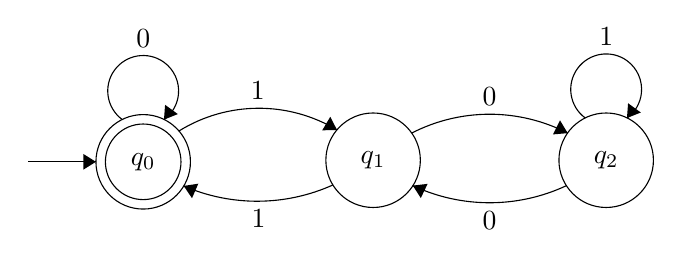
\begin{tikzpicture}[scale=0.2]
        \tikzstyle{every node}+=[inner sep=0pt]
        \draw [black] (21.8,-26.2) circle (3);
        \draw (21.8,-26.2) node {$q_0$};
        \draw [black] (21.8,-26.2) circle (2.4);
        \draw [black] (36.4,-26.1) circle (3);
        \draw (36.4,-26.1) node {$q_1$};
        \draw [black] (51.2,-26.1) circle (3);
        \draw (51.2,-26.1) node {$q_2$};
        \draw [black] (20.477,-23.52) arc (234:-54:2.25);
        \draw (21.8,-18.95) node [above] {$0$};
        \fill [black] (23.12,-23.52) -- (24,-23.17) -- (23.19,-22.58);
        \draw [black] (49.877,-23.42) arc (234:-54:2.25);
        \draw (51.2,-18.85) node [above] {$1$};
        \fill [black] (52.52,-23.42) -- (53.4,-23.07) -- (52.59,-22.48);
        \draw [black] (24.062,-24.248) arc (121.85253:58.93234:9.627);
        \fill [black] (34.11,-24.18) -- (33.68,-23.34) -- (33.17,-24.2);
        \draw (29.08,-22.29) node [above] {$1$};
        \draw [black] (33.852,-27.668) arc (-65.73283:-113.48231:11.715);
        \fill [black] (24.37,-27.73) -- (24.9,-28.51) -- (25.3,-27.59);
        \draw (29.12,-29.21) node [below] {$1$};
        \draw [black] (38.845,-24.378) arc (117.23123:62.76877:10.83);
        \fill [black] (48.76,-24.38) -- (48.27,-23.57) -- (47.82,-24.46);
        \draw (43.8,-22.68) node [above] {$0$};
        \draw [black] (48.68,-27.712) arc (-64.86827:-115.13173:11.491);
        \fill [black] (38.92,-27.71) -- (39.43,-28.5) -- (39.86,-27.6);
        \draw (43.8,-29.3) node [below] {$0$};
        \draw [black] (14.5,-26.2) -- (18.8,-26.2);
        \fill [black] (18.8,-26.2) -- (18,-25.7) -- (18,-26.7);
        \end{tikzpicture}
        \captionof{figure}{Example DFA}
    \end{center}
    \begin{enumerate}
        \item $Q = \{ q_0, q_1, q_2 \}$.
        \item $\Sigma = \{ 0,1 \}$.
        \item $\delta$ is described as: ~
        \begin{center}
            \begin{tabular}{c|cc}
             &0 &1 \\
            \hline
            $q_0$ &$q_0$ & $q_1$ \\
            $q_1$ &$q_2$ & $q_0$\\
            $q_2$ &$q_1$ & $q_2$\\
            \end{tabular}
        \end{center}
        \item $q_0$ is the start state.
        \item $F = \{ q_0 \}$.
    \end{enumerate}
\end{eg}

\begin{definition}[Extended transition function]
    For convenience, we extend $\delta$ to $\bar{\delta}: Q \times \Sigma^{*} \to Q$ inductively as follows:
    \begin{align*}
        \begin{cases}
            \bar{\delta}(q,\epsilon) = q & ~ \\
            \bar{\delta}(q,aw) = \bar{\delta}(\delta(q,a),w) & (a \in \Sigma, w \in \Sigma^{*}) \\
        \end{cases}
    \end{align*}
\end{definition}

\begin{definition} ~
\begin{itemize}
    \item If $\bar{\delta}(q_0, w) \in F$, we say that $w$ is \textbf{accepted} by $\mathcal{M}$.
    \item \textbf{The language accepted by} $\mathcal{M}$ is $L(\mathcal{M}) = \{ w \in \Sigma^{*}: \bar{\delta}(q_0,w)\in F \}$, or we could say that the language accepted by $\mathcal{M}$ is the set of strings accepted by $\mathcal{M}$.
    \item If there is a DFA $\mathcal{M}$ accepts language $L$, we call $L$ is \textbf{DFA-recognizable}.
\end{itemize}
\end{definition}

\subsection{Regular languages} \label{sec:}

\begin{definition}[Regular language]
A language $L$ is regular if $L$ is DFA-recognizable.
\end{definition}

\begin{eg} ~
\begin{itemize}
    \item $L_1 = \{ x \in \Sigma^{*} : x \text{ is the binary representation of multiplier of 3 or } \epsilon \}$ is regular.
    \item $L_2 = \{ 0^{n}1^{n} : n \in \mathbb{N} \}$ is not regular.
\end{itemize}
\end{eg}
\begin{explanation} ~
    \begin{itemize}
        \item $L_1$ is the language accepted by the DFA $\mathcal{M}$ described in Figure 1.1.
        \item Before proving $L_2$ is not regular, we introduce Pumping Lemma.
    \end{itemize}
\end{explanation}

\begin{lemma}[Pumping lemma for regular languages]
Let $L$ be a regular language. Then there exists an integer $p \ge 1$ such that every string $w \in L$ of length at least $p$ can be written as $w = xyz$ satisfying the following conditions:
\begin{itemize}
    \item $|y| \ge 1$
    \item $|xy| \le p$
    \item $\forall n\ge 0$, $xy^{n}z \in L$
\end{itemize}
\end{lemma}
\begin{proof}
For every regular language $L$ there is a DFA accepts it. Let $p = |Q|$, the number of the states. 
\\ For any string $w \in L$ of length at least $p$, then $w$ can be written as $xyz$ such that $\bar{\delta}(q_0,x) = \bar{\delta}(q_0,xy)$, where $|y| \ge 1$ and $|xy|\le p$, as a consequence of pigeonhole principle. (Intuitively, it means that there are $|w|$ states plus one start state visited after transition function finishes, $|w|+1 > p$, so there must be a repeat of states visited during the reading of the first $p$ symbols).
\\ Therefore, by induction we have $\forall n \ge 0$, $\bar{\delta}(q_0,xy^{n}) = \bar{\delta}(q_0,xy) \implies \bar{\delta}(q_0,xy^{n}z) = \bar{\delta}(q_0,xyz) \in F \implies xy^{n}z \in L$.
\end{proof}

\begin{corollary}
    $L_2 = \{ 0^{n}1^{n} : n \in \mathbb{N} \}$ is not regular.
\end{corollary}
\begin{proof}
    For any integer $p\ge 1$, there exists a string $w = 0^{p}1^{p}$ such that for any $x,y,z$ that satisfying $w=xyz$, $|y| \ge 1$, $|xy| \le p$, both $x$ and $y$ has to be a sequence of 0, then let $n = p+1$, $xy^{n}z$ contains $|xy^{p+1}| > p$ 0s in the front which is more than the number of 1s, so $xy^{n}z \not \in L$, hence $L_2$ is not regular.
\end{proof}

\begin{remark}
Note that we proved $L_2$ is not regular by using the contrapositive of pumping lemma in the form:
\\
    If $\forall p \in \mathbb{N}$, $\exists s \in A \text{ with } |s|\ge p$ s.t \\
    $$
    \forall x,y,z \in \Sigma^{*}, (s=xyz \land |y| > 0 \land |xy|\le p) \implies (\exists i \ge 0, \text{ s.t. } xy^iz \notin L)
    $$,
    then $A$ is not regular.
\end{remark}

\newpage
\subsection{Nondeterministic finite automata} \label{sec:}
\begin{definition}[Nondeterministic finite automata] ~
    
    A \textbf{Nondeterministic finite automata (NFA)} is a 5-tuple $\mathcal{M} = (Q, \Sigma, \delta, q_0, F)$,
    \begin{enumerate}
        \item $Q$, $\Sigma$, $q_0$ and $F$ are defined same as in DFA.
        \item $\delta: Q \times \Sigma_\epsilon \to \mathcal{P}(Q)$ is a transition function, where $\Sigma_\epsilon = \Sigma \cup \{ \epsilon \}$
    \end{enumerate}
\end{definition}
\begin{remark} ~
    \begin{itemize}
        \item $\mathcal{P}(Q)$ is the power set of $Q$.
        \item We extended $\Sigma$ with an empty string so that it allows NFA to move from one state to another without reading any symbols.
    \end{itemize}
\end{remark}

\begin{definition}[Extended transition function]
    We extend $\delta$ to $\bar{\delta}: Q \times \Sigma^{*} \to \mathcal{P}(Q)$ as follows:
    \begin{align*}
        \bar{\delta}(q,aw) = \bigcup_{p \in \delta(q,a)} \bar{\delta}(p,w) \qquad (a \in \Sigma, w \in \Sigma^{*})
    \end{align*}
\end{definition}

Similar to $DFA$, we also have the following definitions:
\begin{definition} ~
    \begin{itemize}
        \item If $\bar{\delta}(q_0,w)\cap F \neq \varnothing$, we say that $w$ is \textbf{accepted} by $\mathcal{M}$.
        \item \textbf{The language accepted by} $\mathcal{M}$ is $L(\mathcal{M}) = \{ w \in \Sigma^{*} : \bar{\delta}(q_0,w) \cap F \neq \varnothing \}$.
        \item If there is a NFA $\mathcal{M}$ accepts language $L$, we call $L$ is \textbf{NFA-recognizable}.
    \end{itemize}
\end{definition}

\begin{theorem}[Equivalence of NFAs and DFAs]
    A language $L$ is regular if and only if $L$ is NFA-recognizable. In another word, every NFA has an equivalent DFA, and vise versa.
\end{theorem}
\begin{proof}
$\implies$: Any DFA is a NFA by definition.
\\ $\impliedby$: For a NFA $\mathcal{M} = (Q, \Sigma_\epsilon, \delta, q_0, F)$, construct a DFA $M' = (Q', \Sigma, \delta', q_0', F')$ as follows:
\begin{enumerate}
    \item $Q' = \mathcal{P}(Q)$.
    \item $\delta(A, a) = \bigcup_{q \in A} \delta(q,a)$ with $A \in Q'$.
    \item $q_0' = \{ q_0 \}$.
    \item $F' = \{ A \in Q' : A \cap F \neq \varnothing \}$.
\end{enumerate}
Then $\bar{\delta}(q_0,w) = \bar{\delta'}(q_0', w)$, and thus $L(M) = L(M')$.
\end{proof}

\newpage 
Then we can use the above theorem to prove the closure of regular language under regular operations $\cup$, $\circ$, and $^{*}$:
\begin{lemma} If $A,B \subseteq \Sigma^{*}$ are regular, so is
    \begin{enumerate}
        \item $A \cup B$.
        \item $A \circ B = \{ vw : v \in A, w \in B\}$.
        \item $A^{*} = \{ v_1\circ v_2\circ \cdots\circ v_n : v_i \in A, n \in \mathbb{N}\cup \{ 0 \}\}$
    \end{enumerate}
\end{lemma}
Formal proof omitted, instead we show the idea of the proof:
\begin{proofidea}
For any given $A = L(N_1)$ and $B = L(N_2)$, 
\\ To prove $1$, we construct $N$ as follows:
\begin{figure}[htbp] \centering
    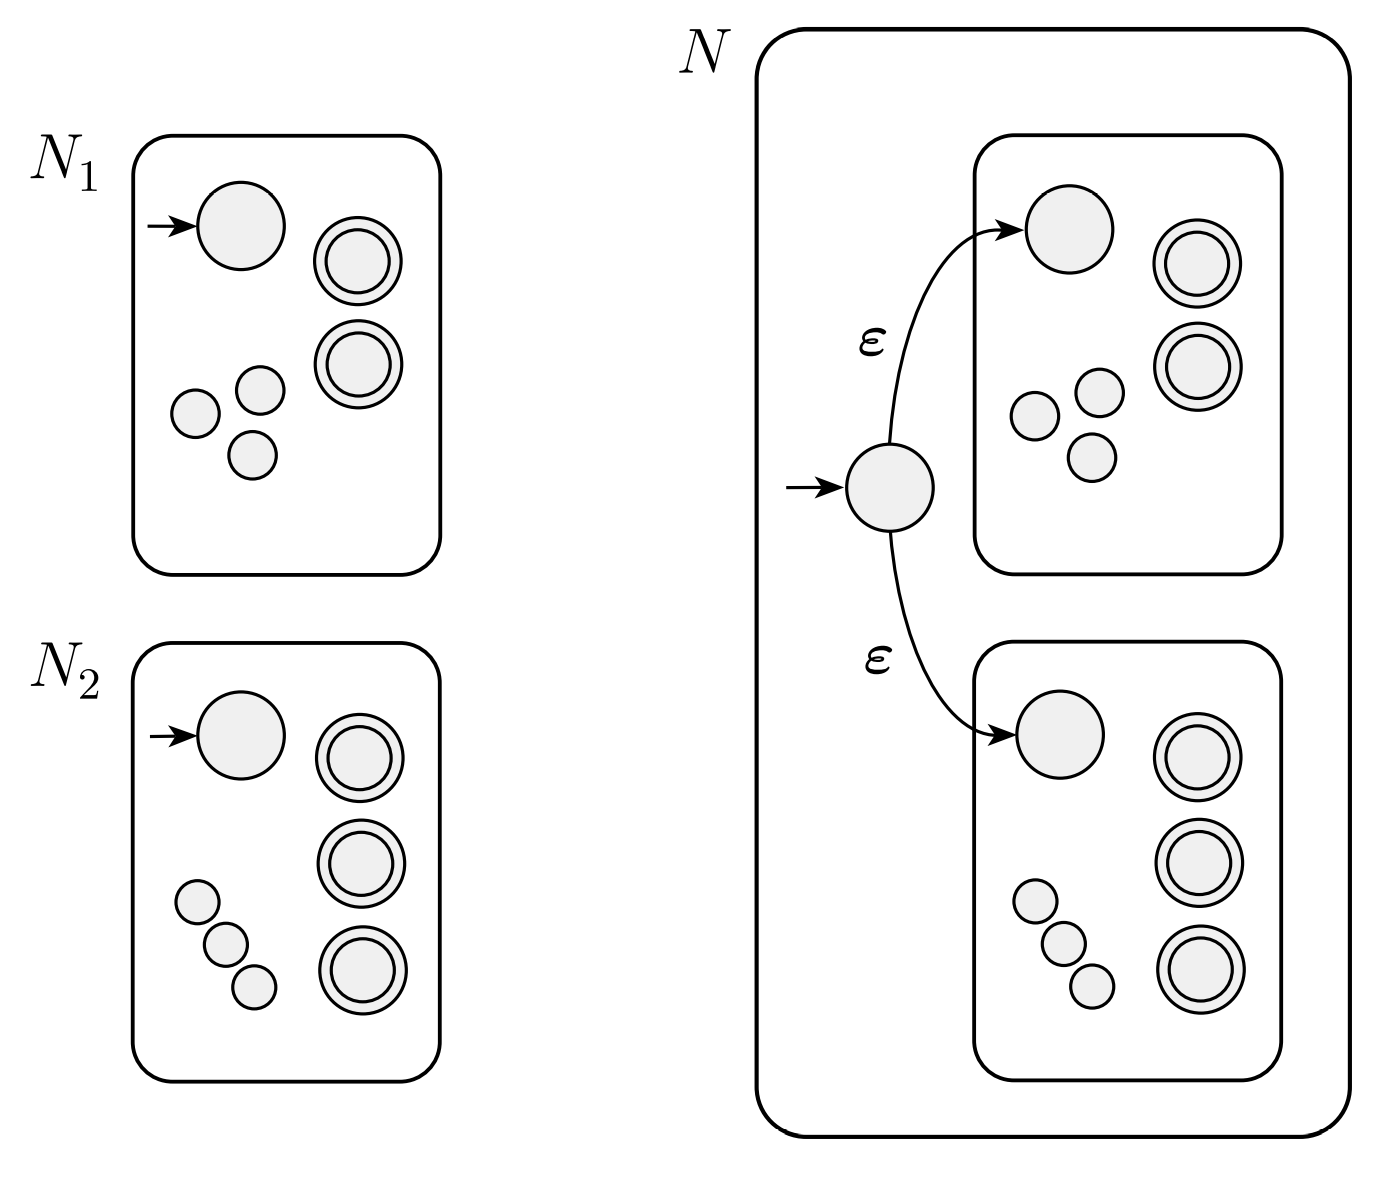
\includegraphics[width=0.5\textwidth]{figures/1.PNG}
    \caption{\label{fig:figure/1.PNG}
        Construction of an NFA $N$ that accepts $A \cup B$. (M. Sipser, 2012)
    }
\end{figure}
\\ To prove $2$, we construct $N$ as follows:
\begin{figure}[htbp] \centering
    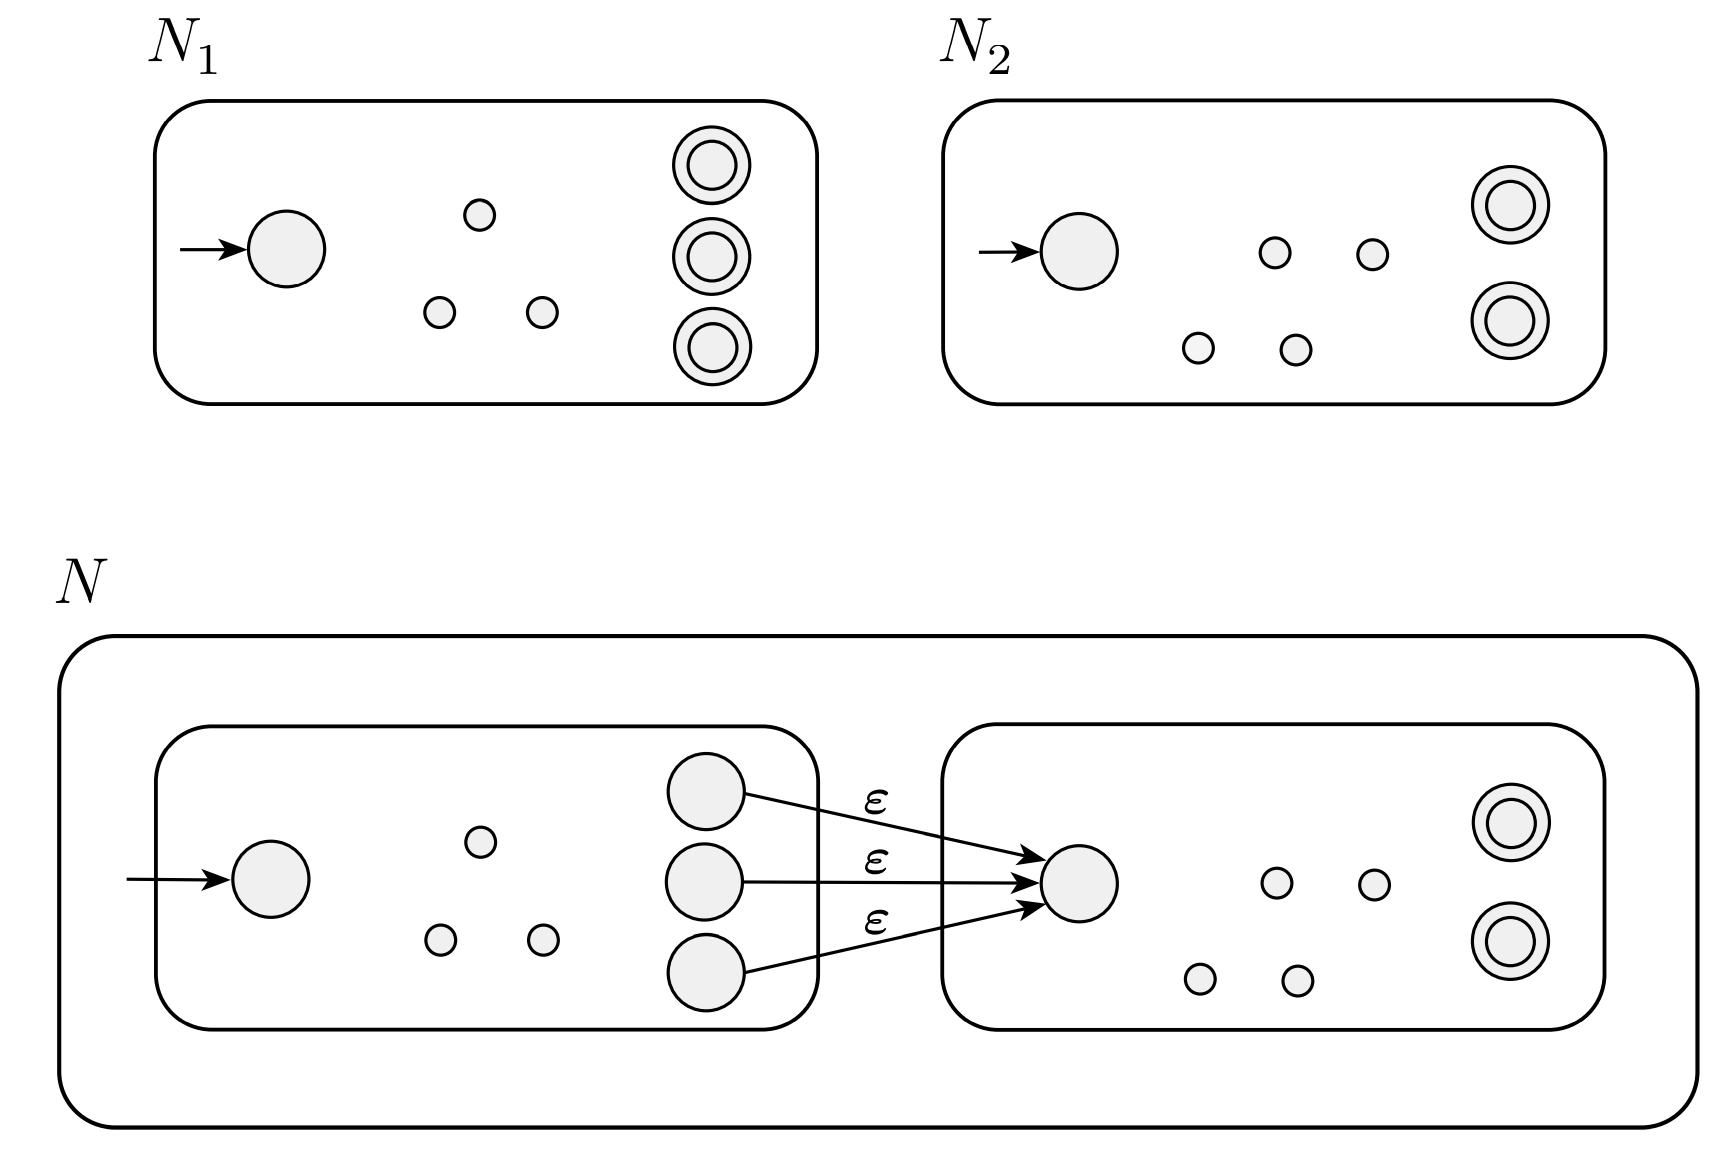
\includegraphics[width=0.5\textwidth]{figures/2.PNG}
    \caption{\label{fig:figure/1.PNG}
        Construction of an NFA $N$ that accepts $A \circ B$. (M. Sipser, 2012)
    }
\end{figure}
\\ To prove $3$, we construct $N$ as follows:
\begin{figure}[htbp] \centering
    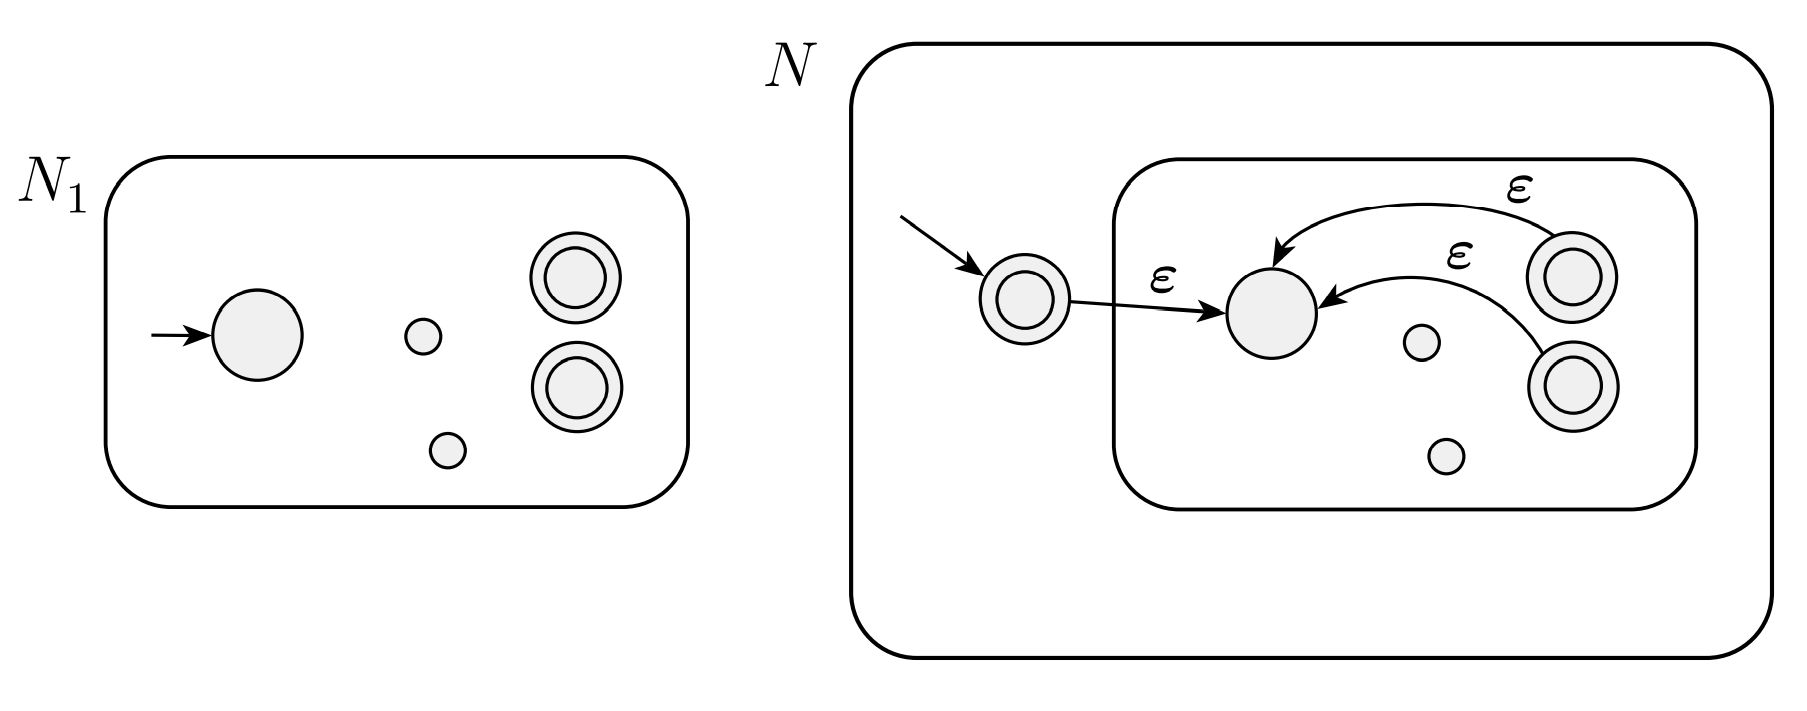
\includegraphics[width=0.5\textwidth]{figures/3.PNG}
    \caption{\label{fig:figure/1.PNG}
        Construction of an NFA $N$ that accepts $A^{*}$. (M. Sipser, 2012)
    }
\end{figure}
\end{proofidea}

\subsection{Regular expressions} \label{sec:}
We define regular expressions inductively:
\begin{definition}[Regular expression]
Say that $R$ is a \textbf{regular expression} is $R$ is
\begin{enumerate}
    \item $\varnothing$,
    \item $\{ \epsilon \}$,
    \item $\{ a \} \subseteq \Sigma$,
    \item $(R_1 \cup R_2)$, where $R_1$ and $R_2$ are regular expressions,
    \item $(R_1 \circ R_2)$, where $R_1$ and $R_2$ are regular expressions, or
    \item $(R_1^{*})$, where $R_1$ is regular expressions.
\end{enumerate}
\end{definition}

The set of NFA-recognizable languages and the set of DFA-recognizable languages are the same according to Theorem 1, but does the set of regular languages same as the set of NFA-recognizable languages? 

Before answering this question, we introduce the generalized nondeterministic finite automaton.
\begin{definition}[generalized nondeterministic finite automaton] ~

A \textbf{generalized nondeterministic finite automaton (GNDF)} is a 5-tuple \\ $\mathcal{M} = (Q,\Sigma,\delta,q_\text{0}, q_\text{accept})$, where
\begin{enumerate}
    \item $Q$, $\Sigma$ and $q_0$ are defined same as in DFA and NFA.
    \item $\delta: (Q\setminus \{ q_0 \}) \times (Q\setminus \{ q_\text{accept} \}) \to \mathcal{R}$ is the transition function, where $\mathcal{R}$ is the collection of all regular expressions over the alphabet $\Sigma$.
    \item $q_\text{accept}$ is the accept state.
\end{enumerate}
\end{definition}
\begin{remark}
    The transition function takes as its argument a pair of two states and outputs a regular expression (the label of the transition).
\end{remark}

Finally, we have a summarized theorem:
\begin{theorem}[Kleene's theorem]
    The set of regular languages, the set of NFA-recognizable languages, and the set of DFA-recognizable languages are all the same.
\end{theorem}

Again, we omit the formal proof but provide the idea of the proof.

\begin{proofidea} Consider the following example reduction from a NFA to a GNFA and then a regular expression:
\begin{figure}[htbp] \centering
    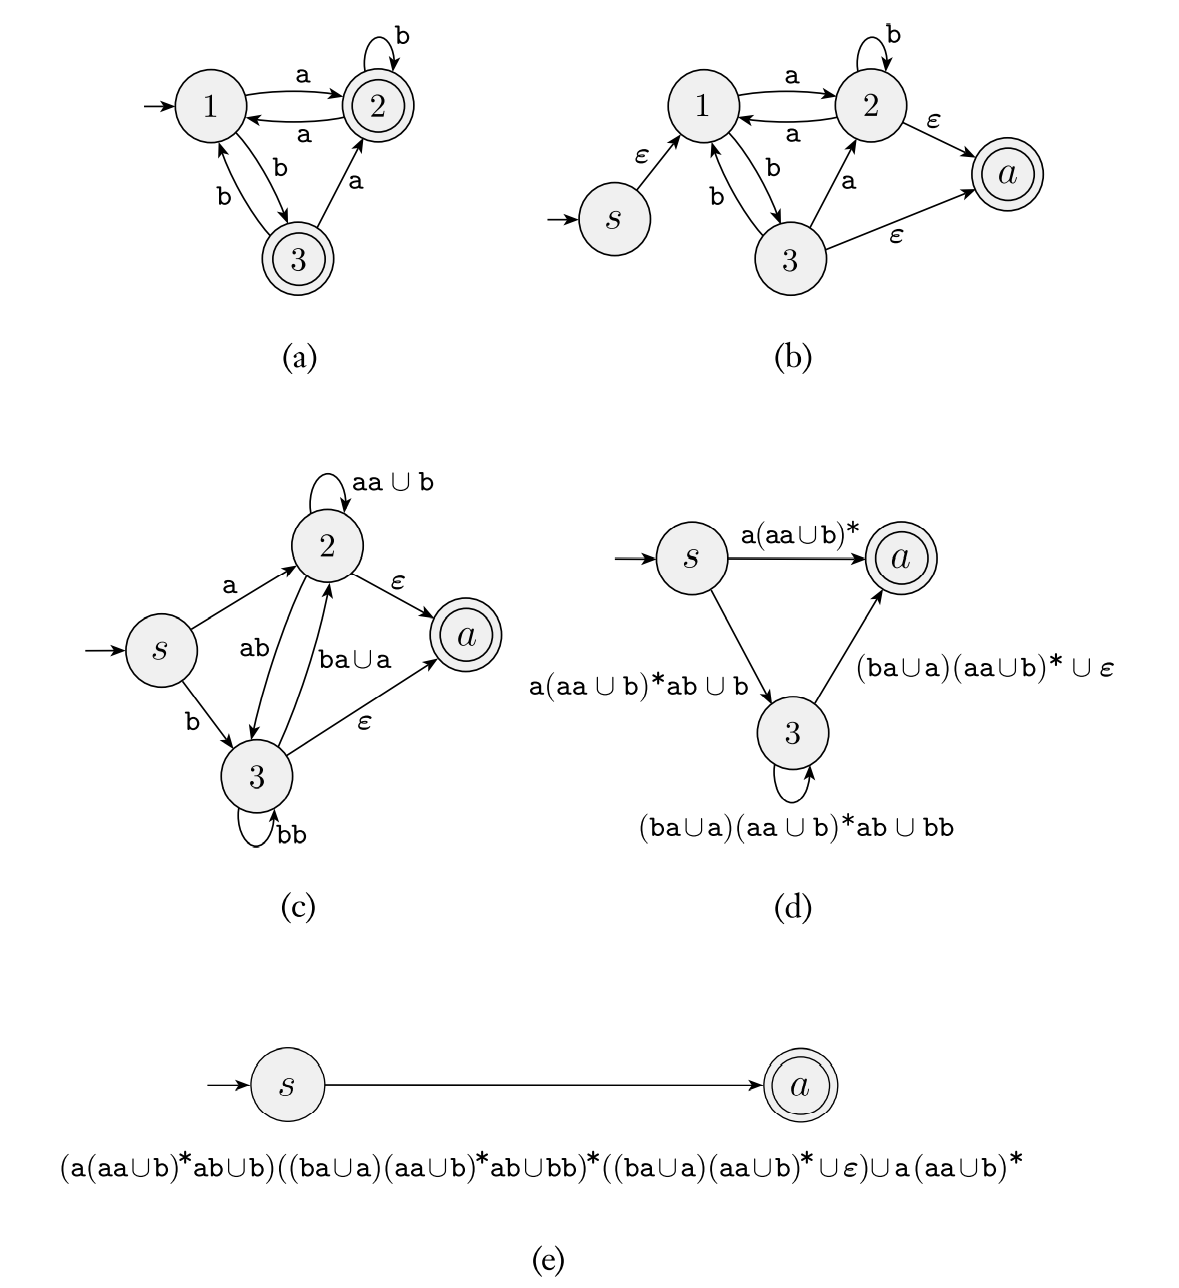
\includegraphics[width=0.7\textwidth]{figures/4.PNG}
    \caption{Converting a three-state DFA to an equivalent regular expression} (M. Sipser, 2012)
\end{figure}
\begin{enumerate}
    \item We first add a new $q_0$ connects to the old $q_0$ and a new $q_\text{accept}$ connects to all the states in $F$.
    \item Then we delete every internal state one by one and append the labels to the corresponding transitions. (After deleting the state $q$, if it has a self-loop labeled with $a$, then we add $a^{*}$ to every path pass through $q$ by squeezing it with the labels at front and back)
\end{enumerate}
\end{proofidea}

\section{Context-Free languages} \label{sec:}
\subsection{Context-Free Grammar} \label{sec:}
Recall that $L = \{ 0^{n}1^{n} : n \in \mathbb{N} \}$ is not regular, equivalent of saying that no regular expression describe it (Kleene's theorem), now we define a more powerful method that can describe this language:
\begin{definition}[Context-free grammars] ~

A \textbf{context-free grammars} is a 4-tuple $G = (V, \Sigma, R, S)$, where
\begin{enumerate}
    \item $V$ is a finite set called the \textbf{variables},
    \item $\Sigma$ is a finite set, disjoint from $V$, called the \textbf{terminals},
    \item $R$ is a finite set of \textbf{rules}, with each rule being a variable and a string of variables and terminals,
    \item $S \in V$ is the start variable.
\end{enumerate}
\end{definition}


\begin{definition}[Rule] ~
    \begin{itemize}
        \item 
    \end{itemize}
\end{definition}


\begin{eg}
Consider grammar $G = (\{ S \}, \{ 0, 1 \}, R, S)$. The set of rules, $R$, is
\begin{align*}
    S \to 0S1 | \epsilon
\end{align*}
\end{eg}




